\documentclass[conference,a4paper]{IEEEtran}

\usepackage{cite}
\usepackage{amsmath,amssymb,amsfonts}
\usepackage{graphicx}
\usepackage{textcomp}
\usepackage{xcolor}
\usepackage{booktabs}
\usepackage{url}

\def\BibTeX{{\rm B\kern-.05em{\sc i\kern-.025em b}\kern-.08em
    T\kern-.1667em\lower.7ex\hbox{E}\kern-.125emX}}

\begin{document}

\title{Machine Learning-Based Prediction of Tourist Arrivals in Sri Lanka Using Economic, Environmental, and Tourism Factors}

\author{\IEEEauthorblockN{RPJLK Rajapaksha}
\IEEEauthorblockA{\textit{Electrical and Telecommunications Engineering} \\
\textit{General Sir John Kotelawala Defence University}\\
Ratmalana, Sri Lanka \\
jlkrajapaksha@gmail.com}}

\maketitle

\begin{abstract}
Accurate forecasts of tourist arrivals can support planning and resource allocation in the tourism sector. This study investigates the prediction of monthly tourist arrivals to Sri Lanka from individual origin countries using economic, environmental, and tourism-related variables. A dataset containing 750 observations from 2018 to 2024 was prepared for a supervised regression task. Numerical attributes were standardized and categorical attributes were one-hot encoded. Two evaluation strategies were compared: a chronological split for realistic future-year forecasting and a random split containing 70 percent training data, 15 percent validation data, and 15 percent test data for interpolation within the observed period. Linear Regression, second-degree Polynomial Regression, and radial basis function Support Vector Regression were evaluated using mean absolute error, mean squared error, root mean squared error, and R-squared. On the chronological 2024 test set, Linear Regression achieved a mean absolute error of 5,011.12, a root mean squared error of 6,729.14, and an R-squared score of 0.546, while Support Vector Regression obtained a negative R-squared score of -0.470. Under random testing, Support Vector Regression instead achieved a root mean squared error of 4,064.67 and an R-squared score of 0.835. This large difference is attributed to temporal distribution shift: the chronological training data combine pre-pandemic demand, the COVID-19 collapse, and early recovery, whereas 2023 and 2024 follow a later and different recovery pattern. Random splitting mixes these regimes and therefore produces more optimistic results that do not represent genuine future-year forecasting.
\end{abstract}

\begin{IEEEkeywords}
tourist arrivals, machine learning, linear regression, polynomial regression, support vector regression, Sri Lanka
\end{IEEEkeywords}

\section{Introduction}
Tourism is an important contributor to the Sri Lankan economy, and changes in international arrivals affect accommodation demand, transport services, employment, and public-sector planning. However, arrivals vary with season, origin country, economic conditions, environmental conditions, and unexpected disruptions. Estimating future demand from these factors is therefore a useful regression problem.

This study develops and evaluates machine-learning models that predict the monthly number of tourists arriving in Sri Lanka from a given origin country. The main objectives are to: (1) examine the structure and quality of the selected dataset; (2) prepare economic, environmental, and tourism-related variables for modeling; (3) train Linear Regression, Polynomial Regression, and Support Vector Regression (SVR) models; and (4) compare chronological future-year evaluation with randomized interpolation to determine how the split strategy affects reported performance.

The remainder of this paper is organized as follows. Section II describes the dataset, exploratory analysis, preprocessing, experimental design, and models. Section III presents the evaluation results and their interpretation. Section IV discusses strengths, limitations, and practical implications, while Section V concludes the paper and identifies possible future improvements.

\section{Methodology}

\subsection{Dataset Description}
The dataset contains 750 observations and 13 original variables covering the period from 2018 to 2024 \cite{peasinghe_tourist_dataset}. Each observation represents the tourist arrivals recorded for an origin country in a particular month. One variable, \texttt{totalCount}, is the response, leaving 12 candidate predictor features. These predictors are year, month, origin country, exchange rate, mean apparent temperature, sunshine duration, rainfall, precipitation hours, number of tourism establishments, number of rooms, an air-passenger fares index, and a consumer price index.

The target ranges from 10 to 52,881 arrivals, with a mean of 8,621.44 and a standard deviation of 9,127.99. This difference between the mean and standard deviation, together with the observed histogram, indicates a wide and right-skewed target distribution. No missing values or duplicate rows were detected. The dataset source and the original sources of its economic, weather, and tourism variables must be cited in the final version of the paper. % TODO: Add verified dataset-source citations.

\begin{table}[htbp]
\caption{Dataset and Experimental Split}
\label{tab:dataset-split}
\centering
\begin{tabular}{lcc}
\toprule
\textbf{Subset} & \textbf{Period} & \textbf{Observations} \\
\midrule
Training & 2018--2022 & 510 \\
Validation & 2023 & 120 \\
Testing & 2024 & 120 \\
\midrule
Total & 2018--2024 & 750 \\
\bottomrule
\end{tabular}
\end{table}

\subsection{Exploratory Data Analysis}
Exploratory analysis \cite{tukey1977eda} examined the target distribution, total arrivals over time, the leading origin countries, monthly seasonality, and correlations between numerical variables and the target. Among the numerical predictors, the air-passenger fares index showed the strongest positive linear correlation with arrivals ($r=0.241$), while precipitation hours showed the strongest negative correlation ($r=-0.255$). These correlations are modest and do not account for the categorical effect of origin country, but they suggest that both economic and seasonal conditions are relevant. The time series also contains the sharp changes associated with the COVID-19 period, making generalization to later years challenging.

Fig.~\ref{fig:target-distribution} confirms that arrival counts are right-skewed: most country-month observations are concentrated at lower values, while a smaller number of high-volume observations form a long upper tail. This variation explains why RMSE is consistently higher than MAE, since RMSE places more weight on the comparatively large errors made for high-arrival observations.

\begin{figure}[htbp]
\centering
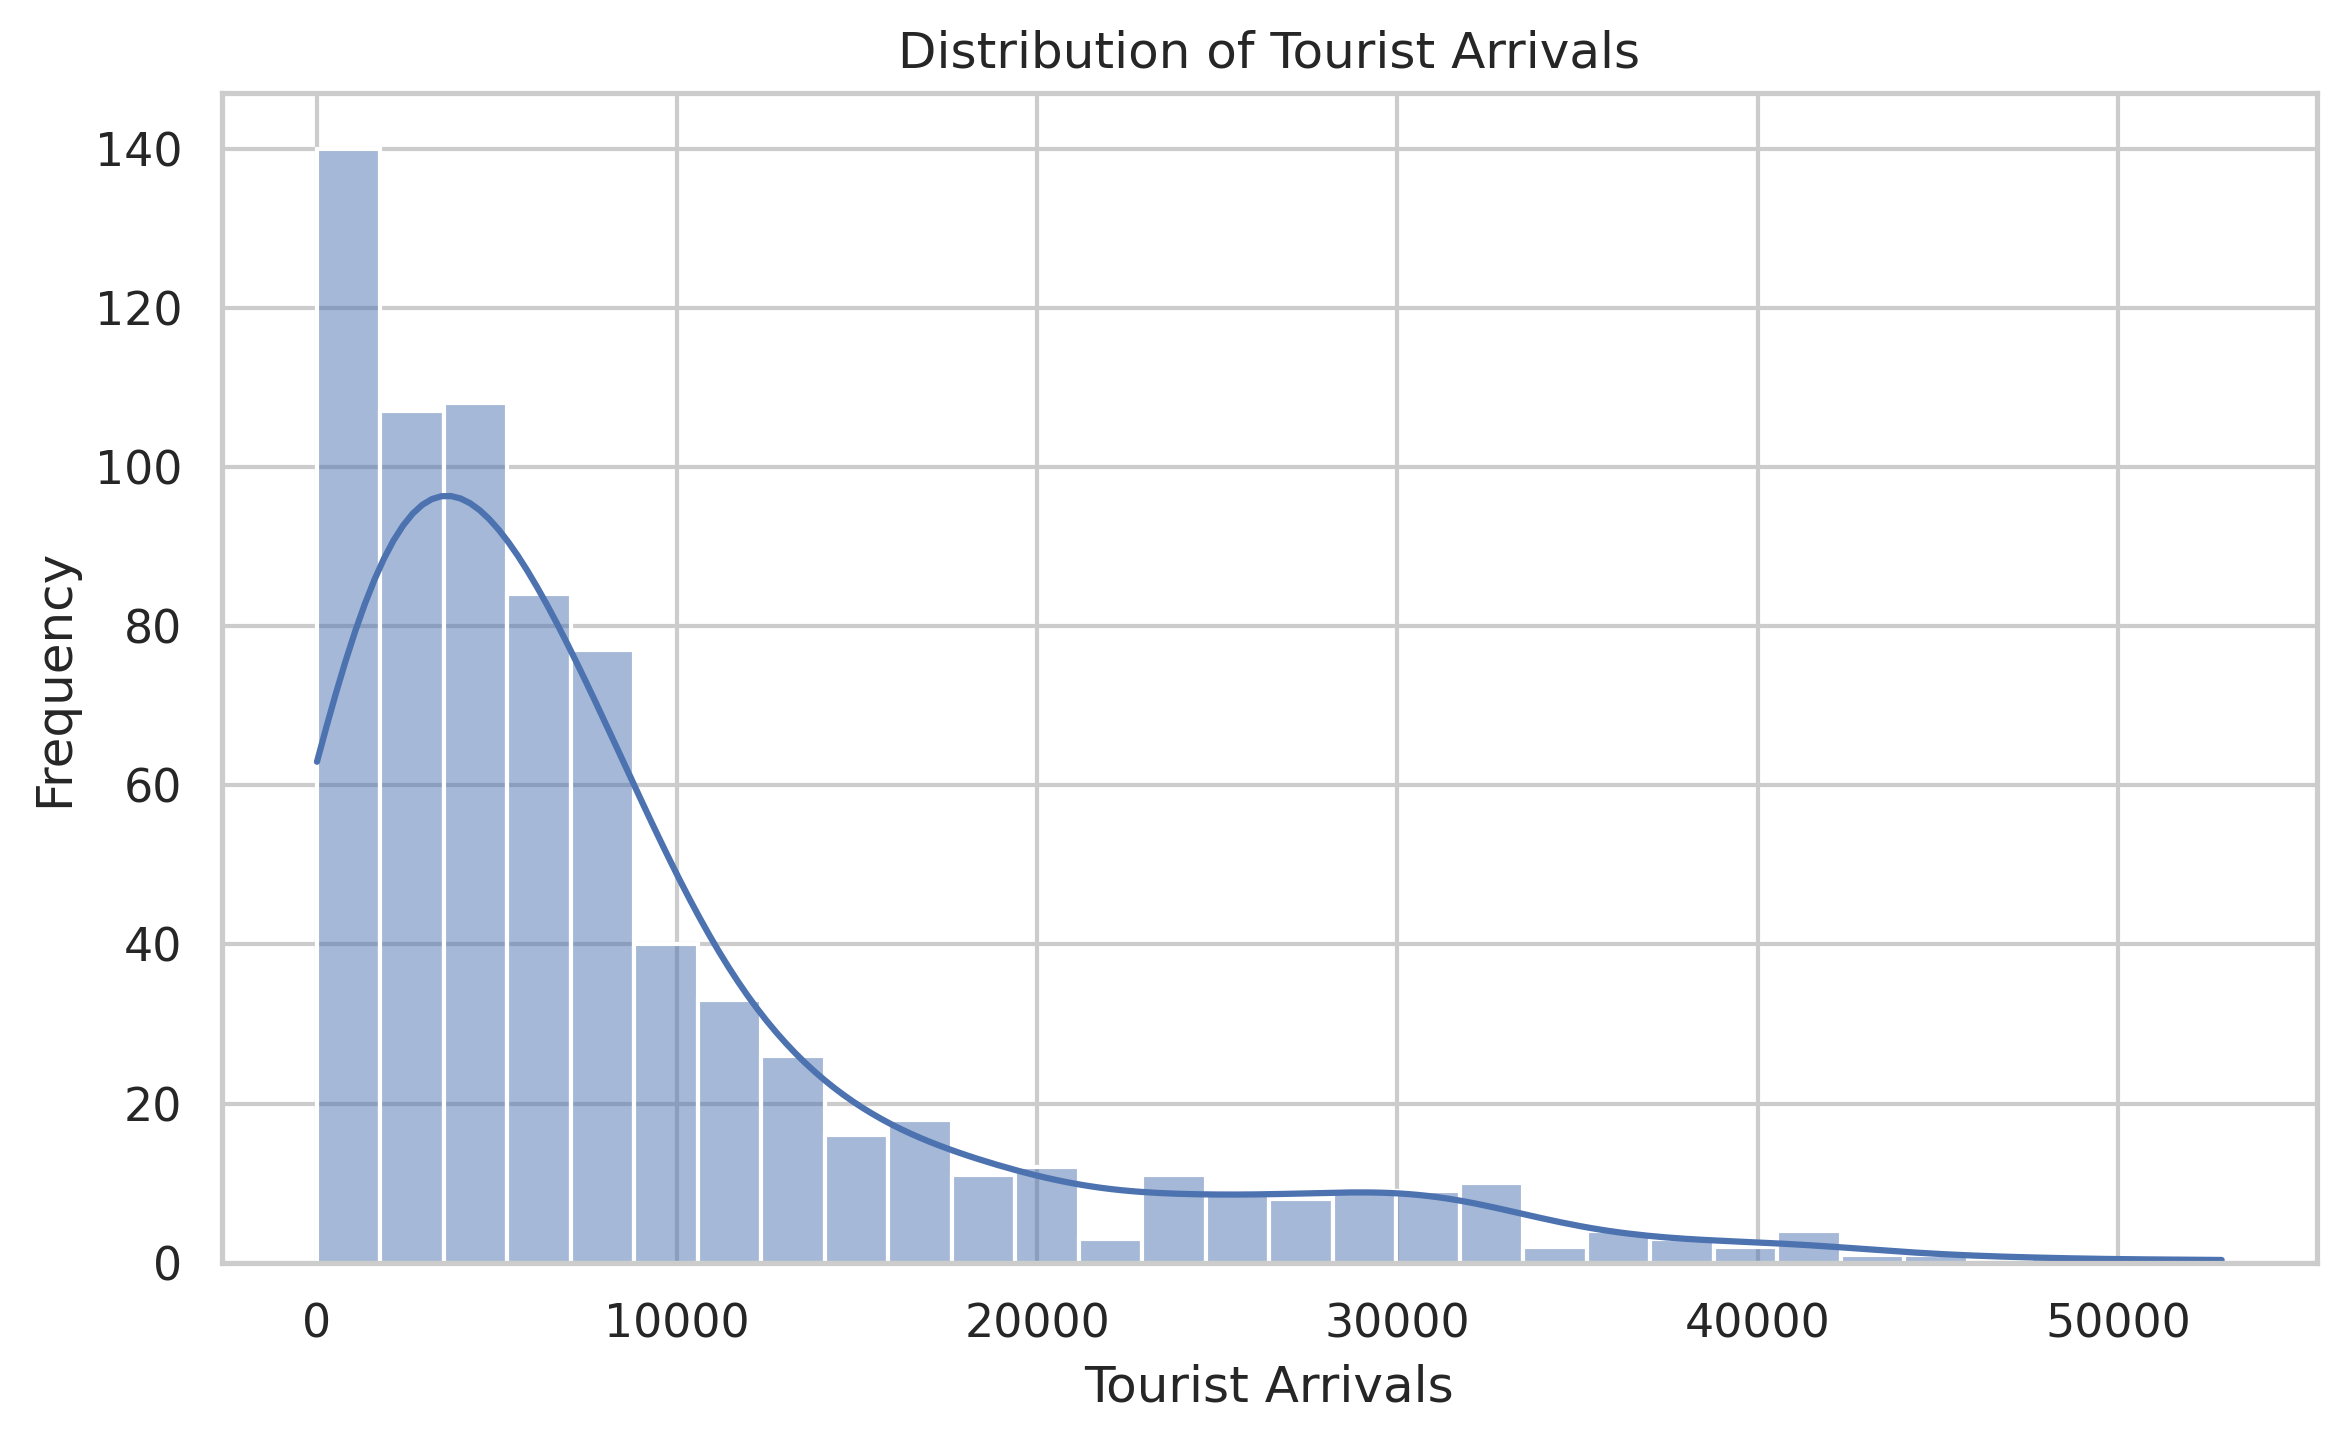
\includegraphics[width=\columnwidth]{figures/target_distribution.png}
\caption{Frequency distribution of monthly tourist-arrival counts across all country-month observations.}
\label{fig:target-distribution}
\end{figure}

The distribution by origin country is shown in Fig.~\ref{fig:country-distribution}. India contributes the largest cumulative number of arrivals in the dataset, followed by the United Kingdom and Russia. The pronounced differences among countries show that the target is also imbalanced across origin markets. This supports treating origin country as a categorical predictor and helps explain why a single global model can produce larger errors for high-volume countries.

\begin{figure}[htbp]
\centering
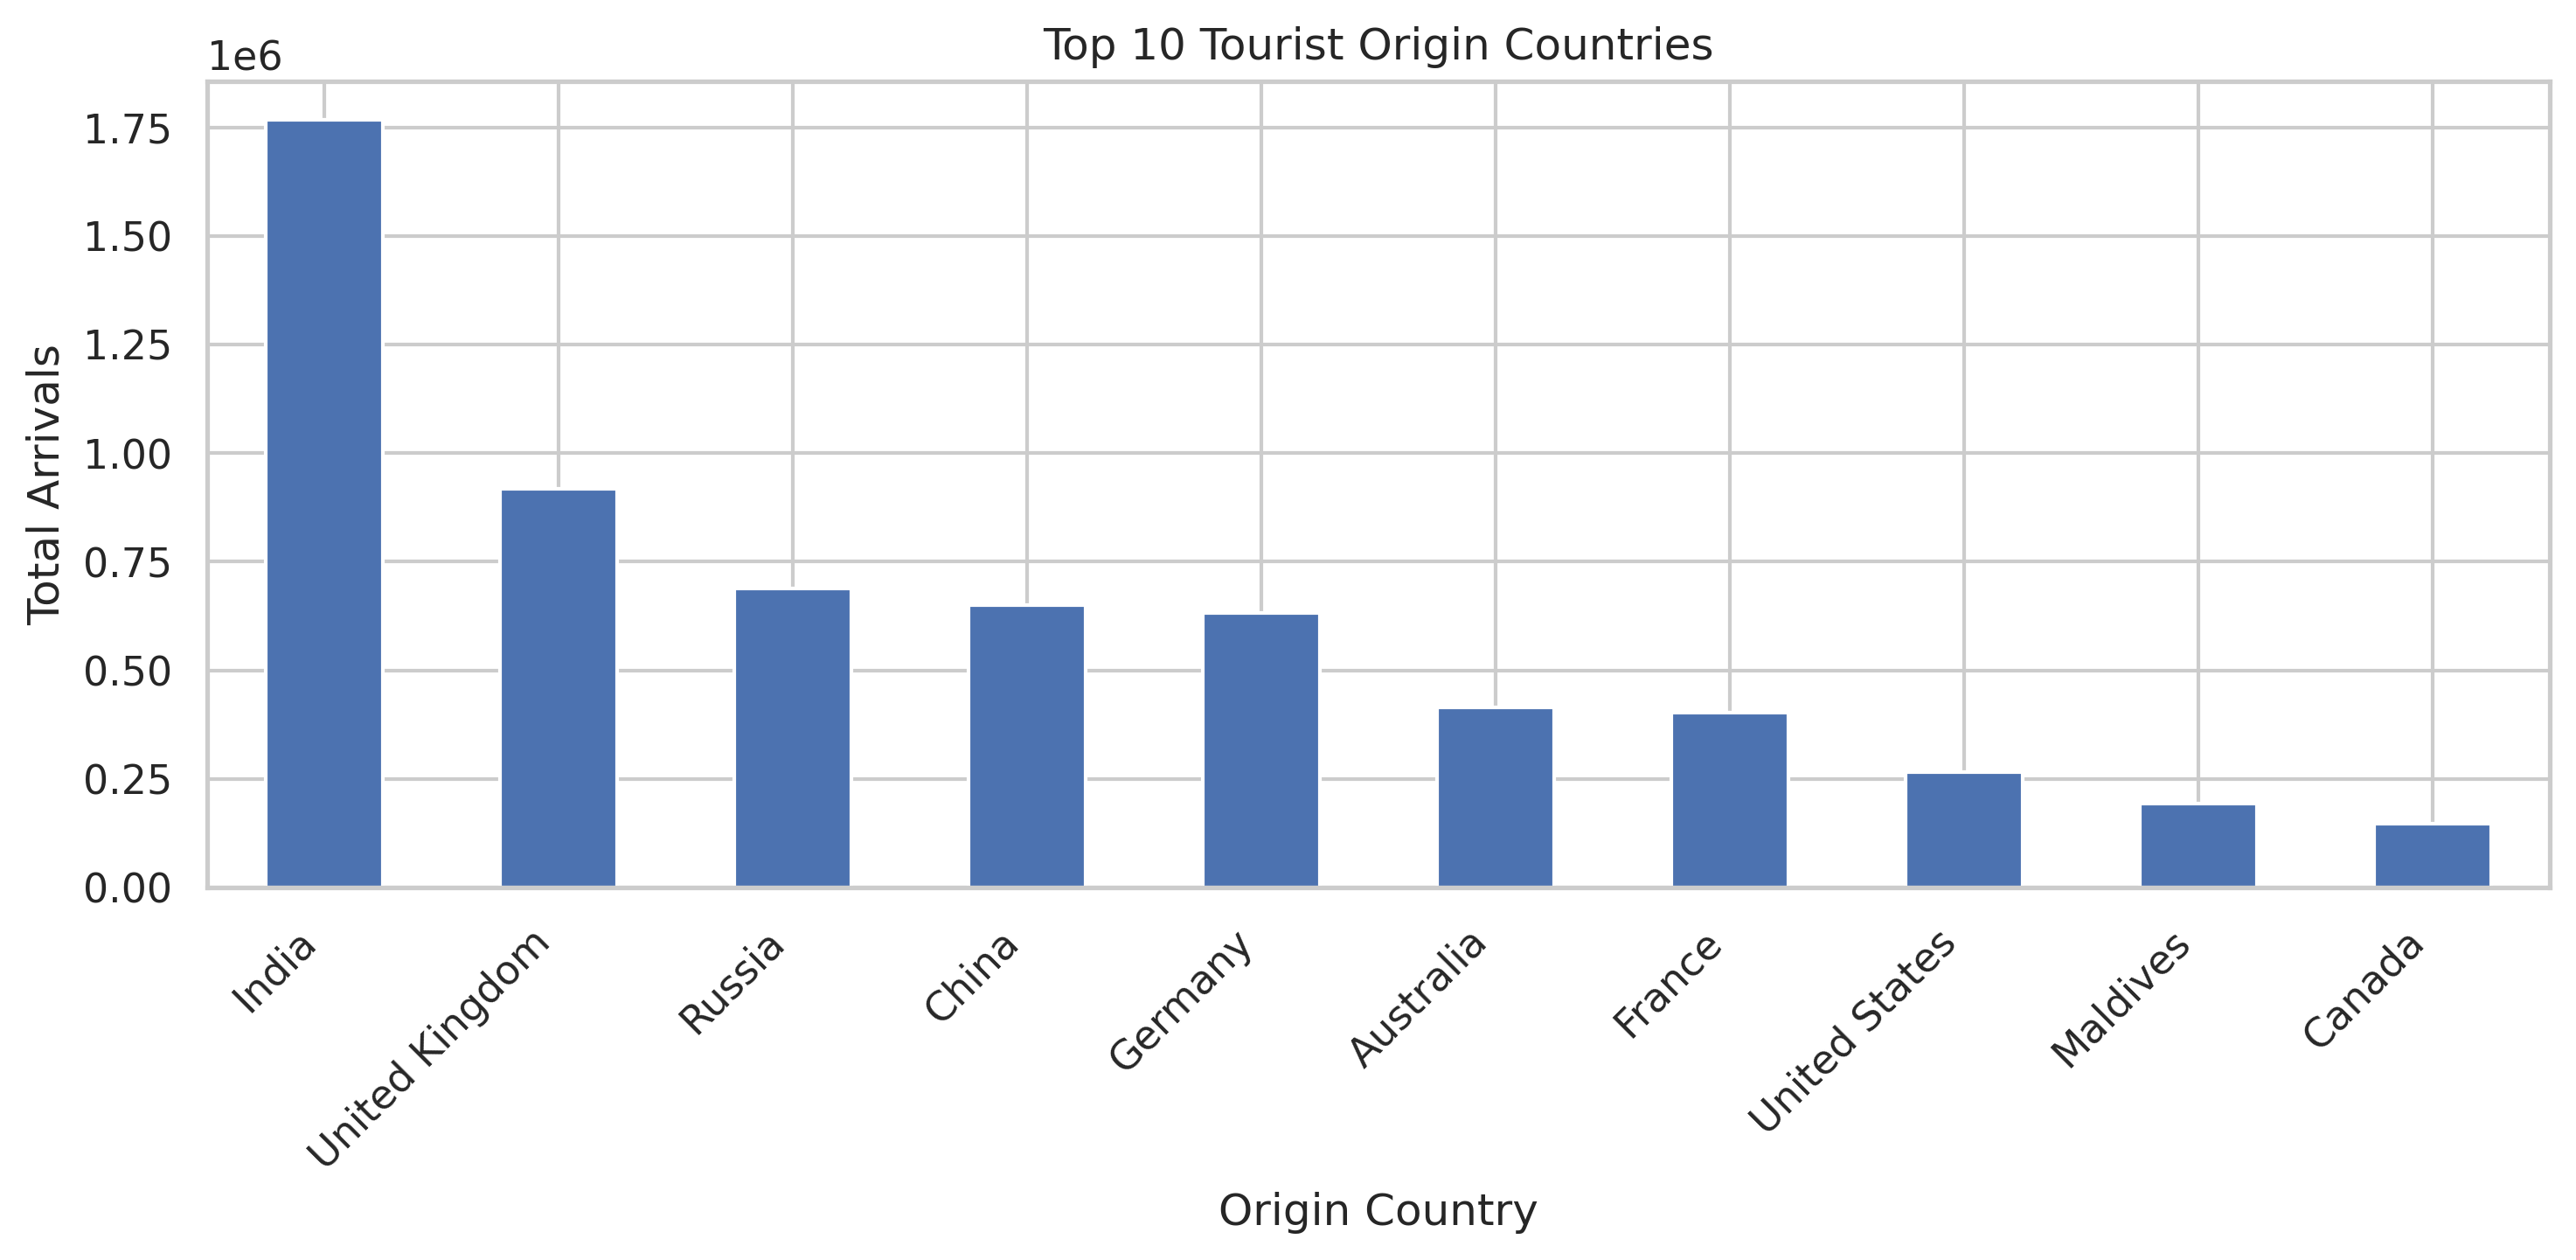
\includegraphics[width=\columnwidth]{figures/top_origin_countries.png}
\caption{Total tourist arrivals from the ten leading origin countries in the dataset.}
\label{fig:country-distribution}
\end{figure}

Fig.~\ref{fig:feature-correlations} compares the individual Pearson correlations between each numerical predictor and tourist arrivals. The air-passenger fares index has the strongest positive correlation, while precipitation hours has the strongest negative correlation. However, all coefficients are relatively modest. The graph therefore indicates that no single numerical predictor explains tourist arrivals adequately and that the models must combine temporal, economic, environmental, capacity, and origin-country information.

\begin{figure*}[htbp]
\centering
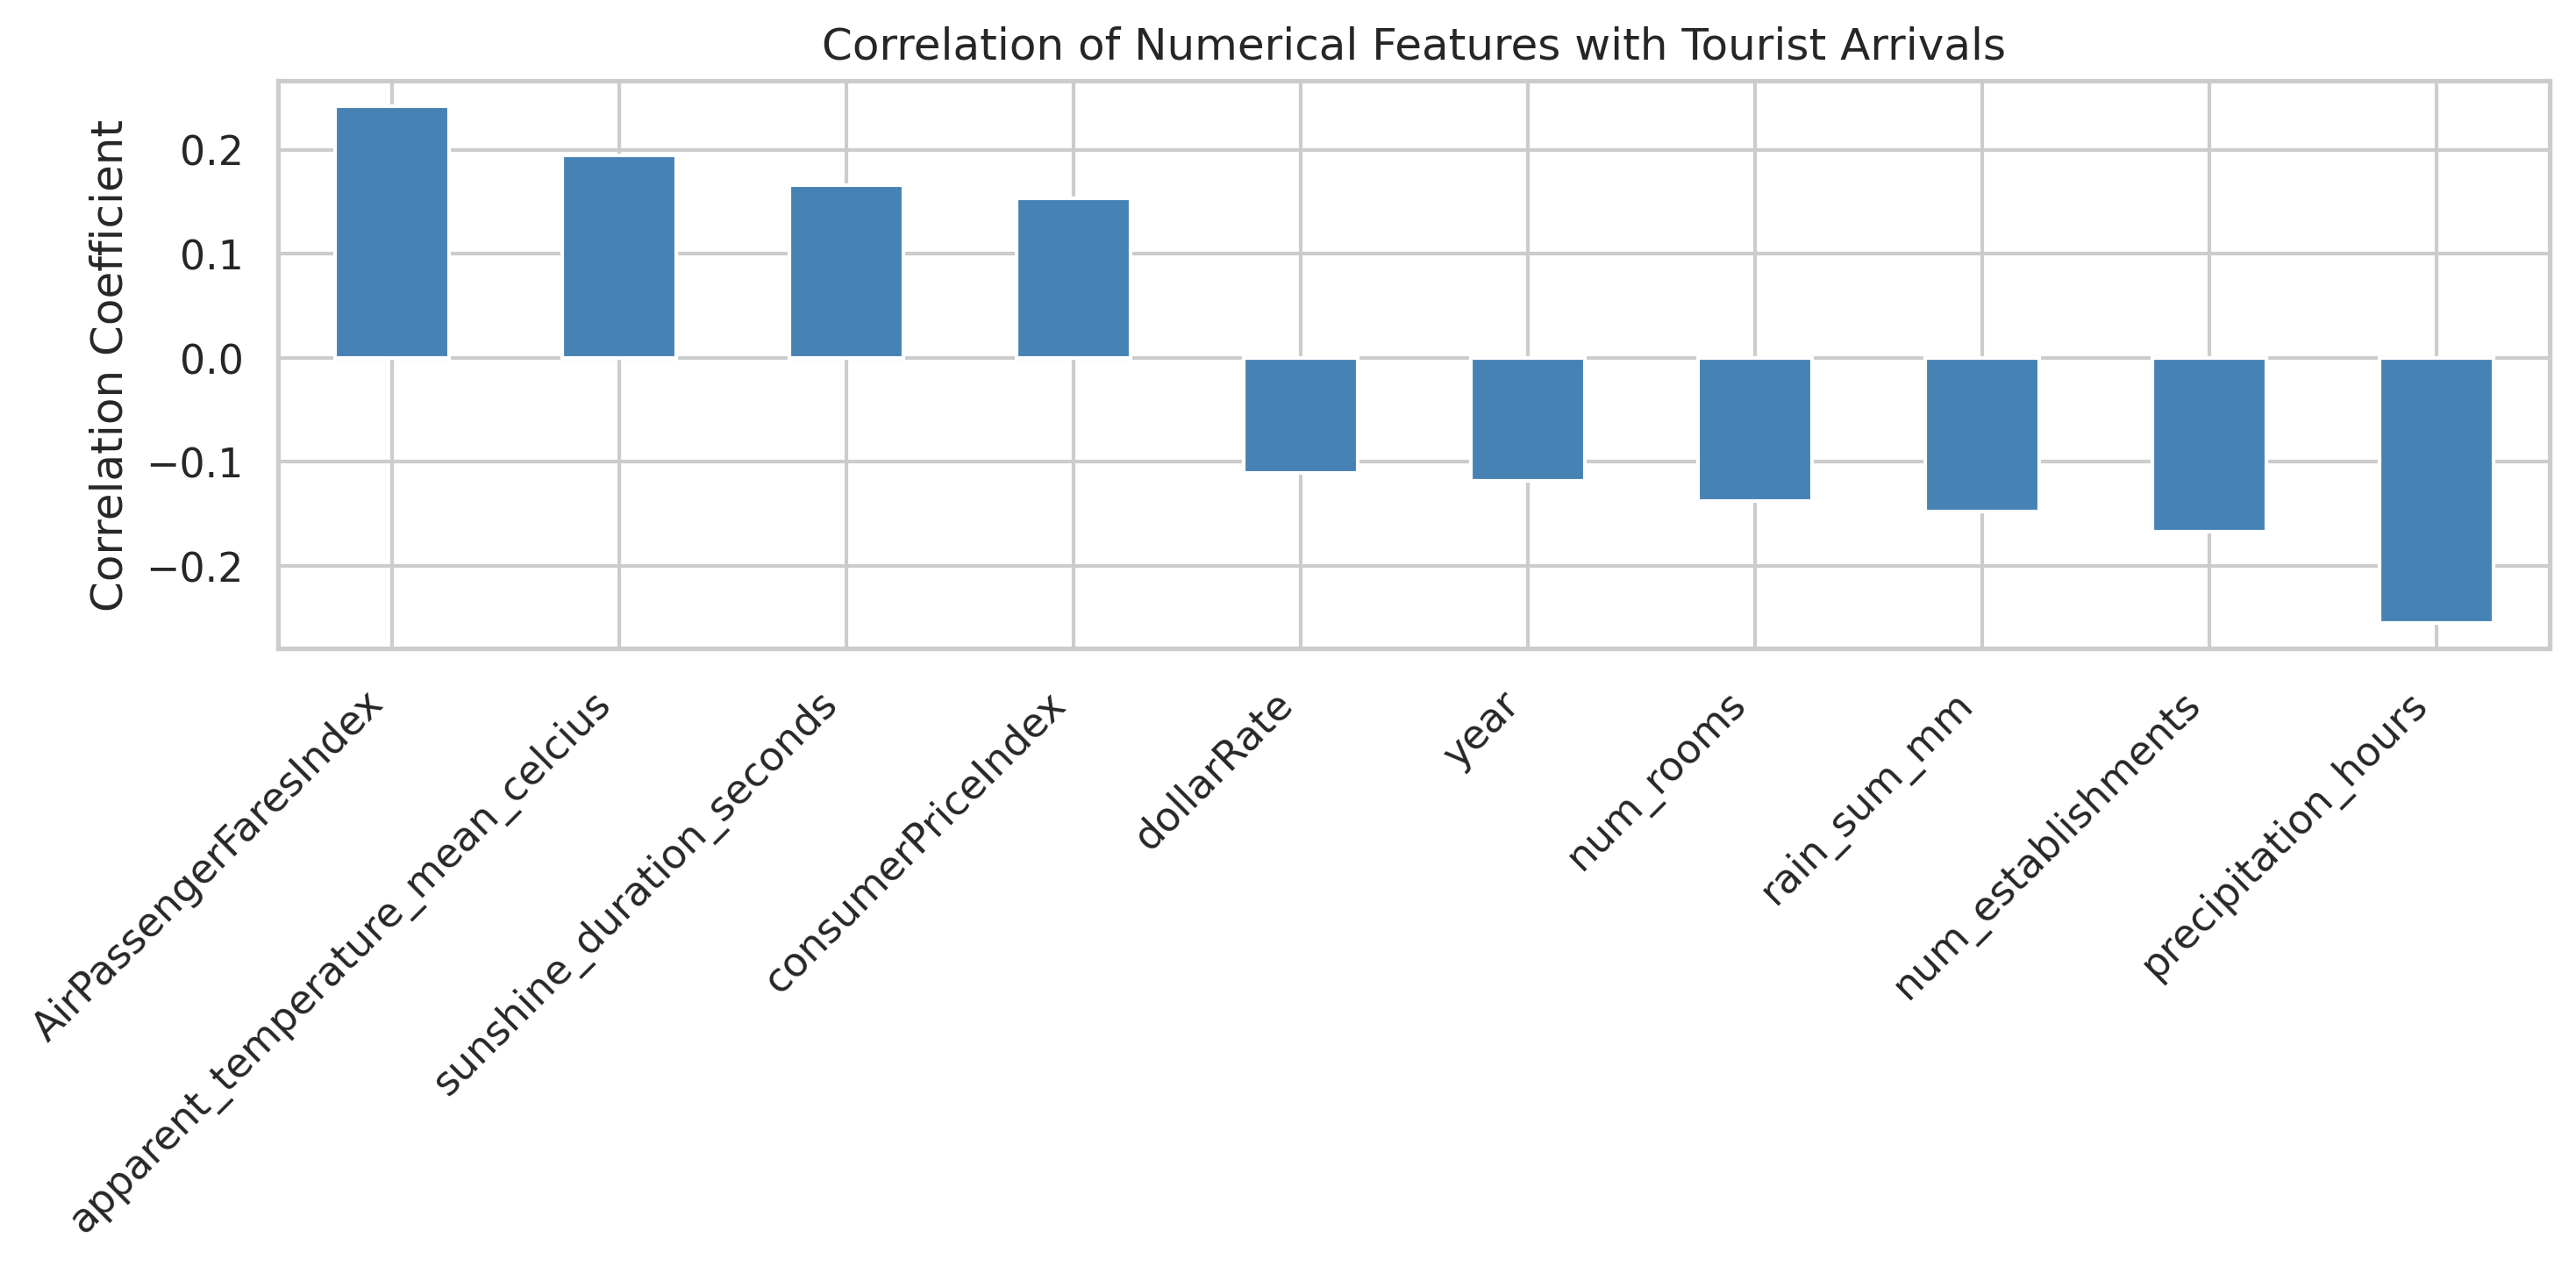
\includegraphics[width=0.86\textwidth]{figures/target_feature_correlations.png}
\caption{Pearson correlations between numerical predictors and tourist arrivals.}
\label{fig:feature-correlations}
\end{figure*}

The monthly totals in Fig.~\ref{fig:arrival-timeline} expose the main temporal challenge in the dataset. Arrivals were relatively high before the pandemic, collapsed during the COVID-19 travel restrictions, and then recovered progressively. The later recovery does not simply reproduce the earlier pattern, so observations in 2023 and 2024 are drawn from a different temporal regime from much of the training data.

\begin{figure*}[htbp]
\centering
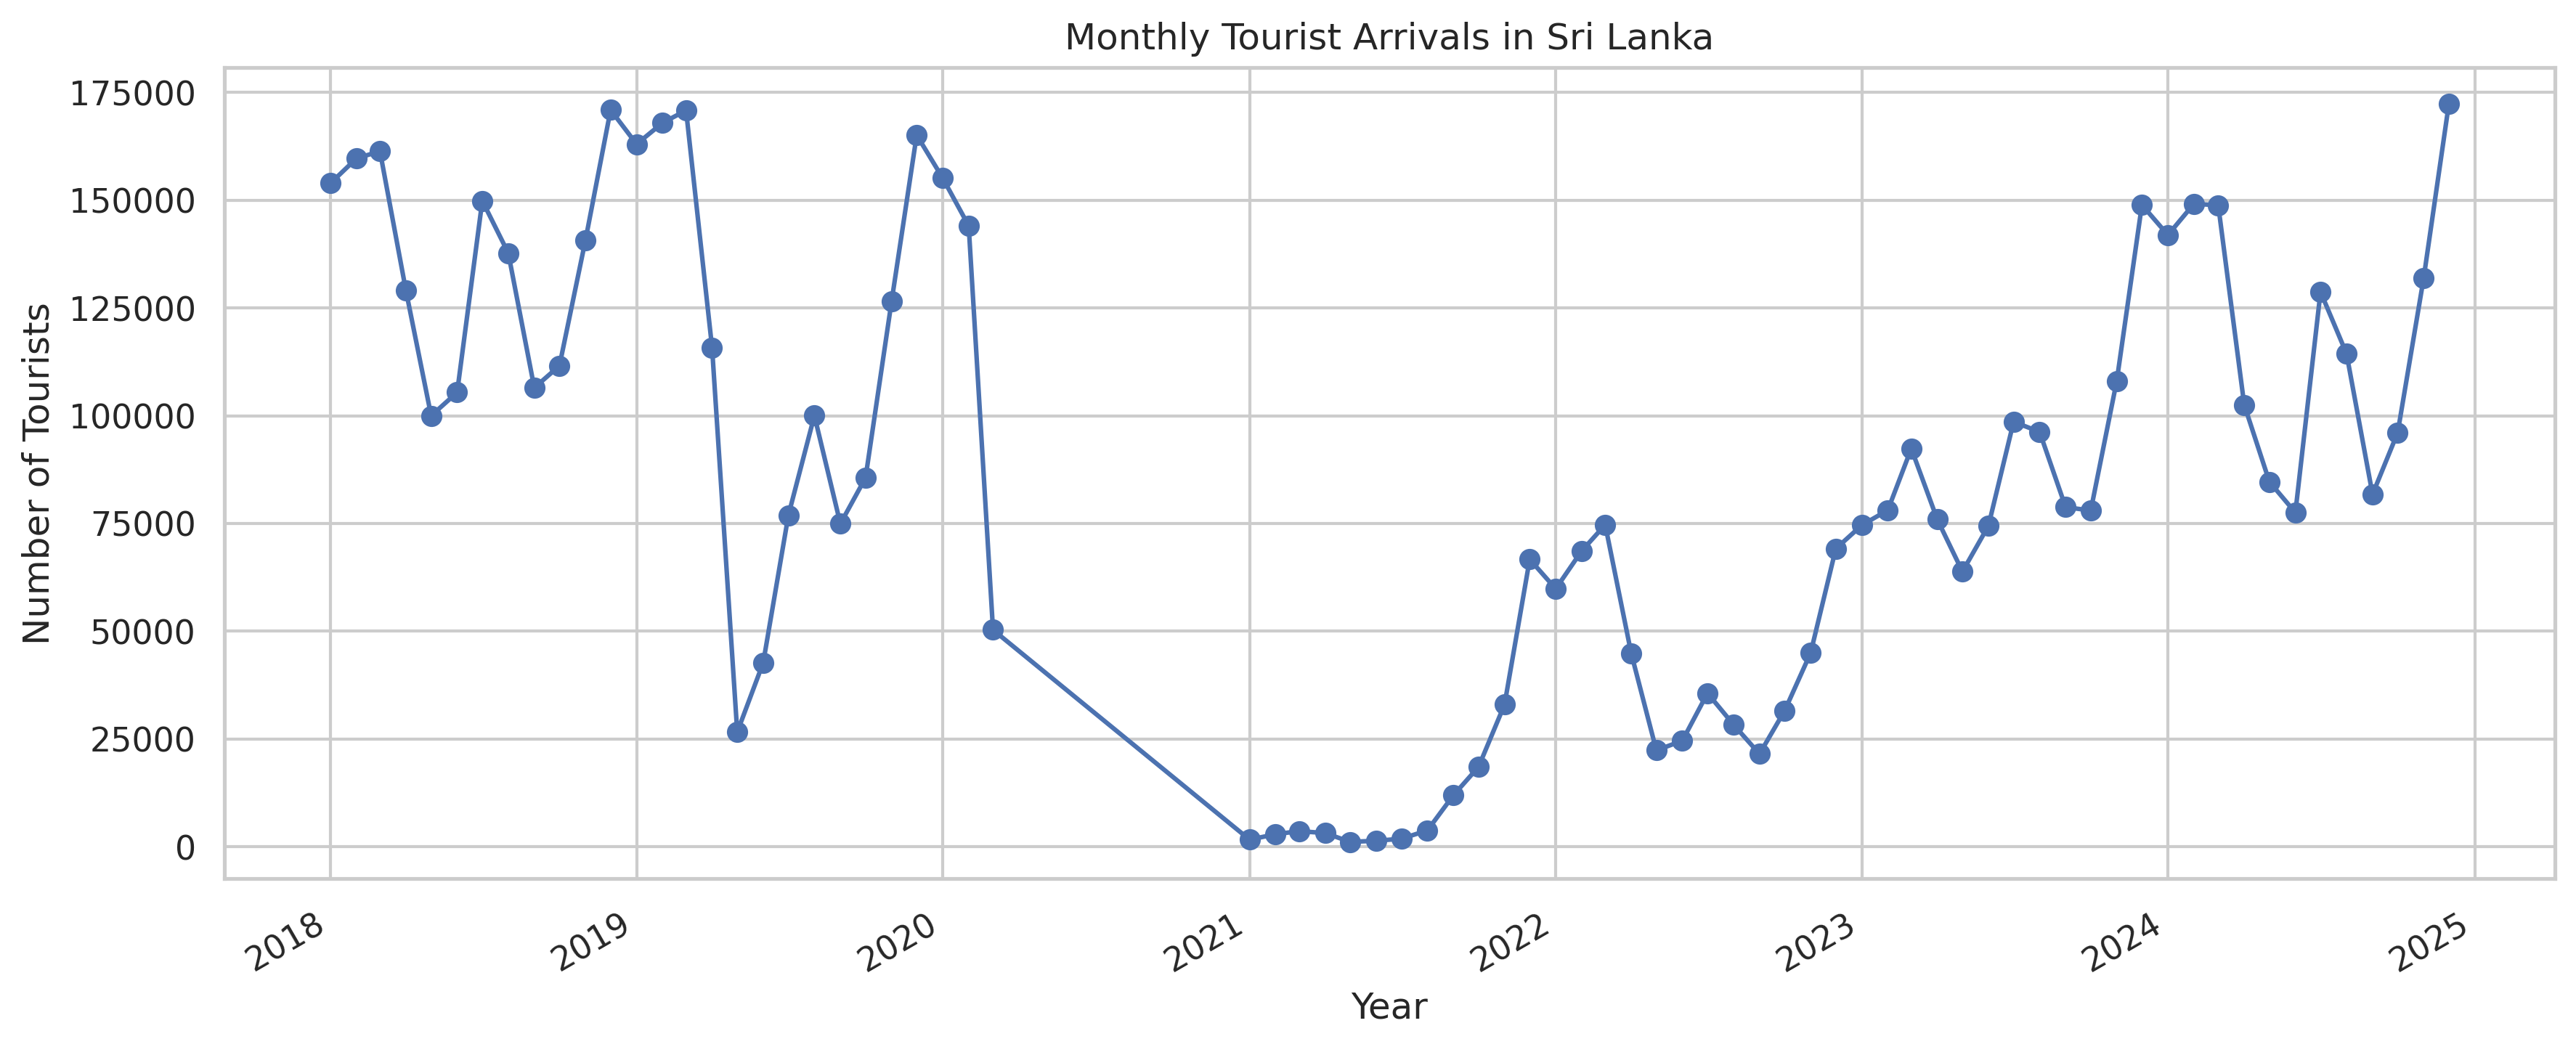
\includegraphics[width=0.88\textwidth]{figures/monthly_arrivals_timeline.png}
\caption{Monthly tourist arrivals over the 2018--2024 study period, showing the COVID-19 collapse and subsequent recovery.}
\label{fig:arrival-timeline}
\end{figure*}

Fig.~\ref{fig:seasonal-boxplot} shows that both the median and spread of arrivals vary across calendar months. However, substantial overlap remains among the monthly distributions, indicating that month alone cannot explain the target and motivating the inclusion of country, economic, environmental, and tourism-capacity predictors.

\begin{figure}[htbp]
\centering
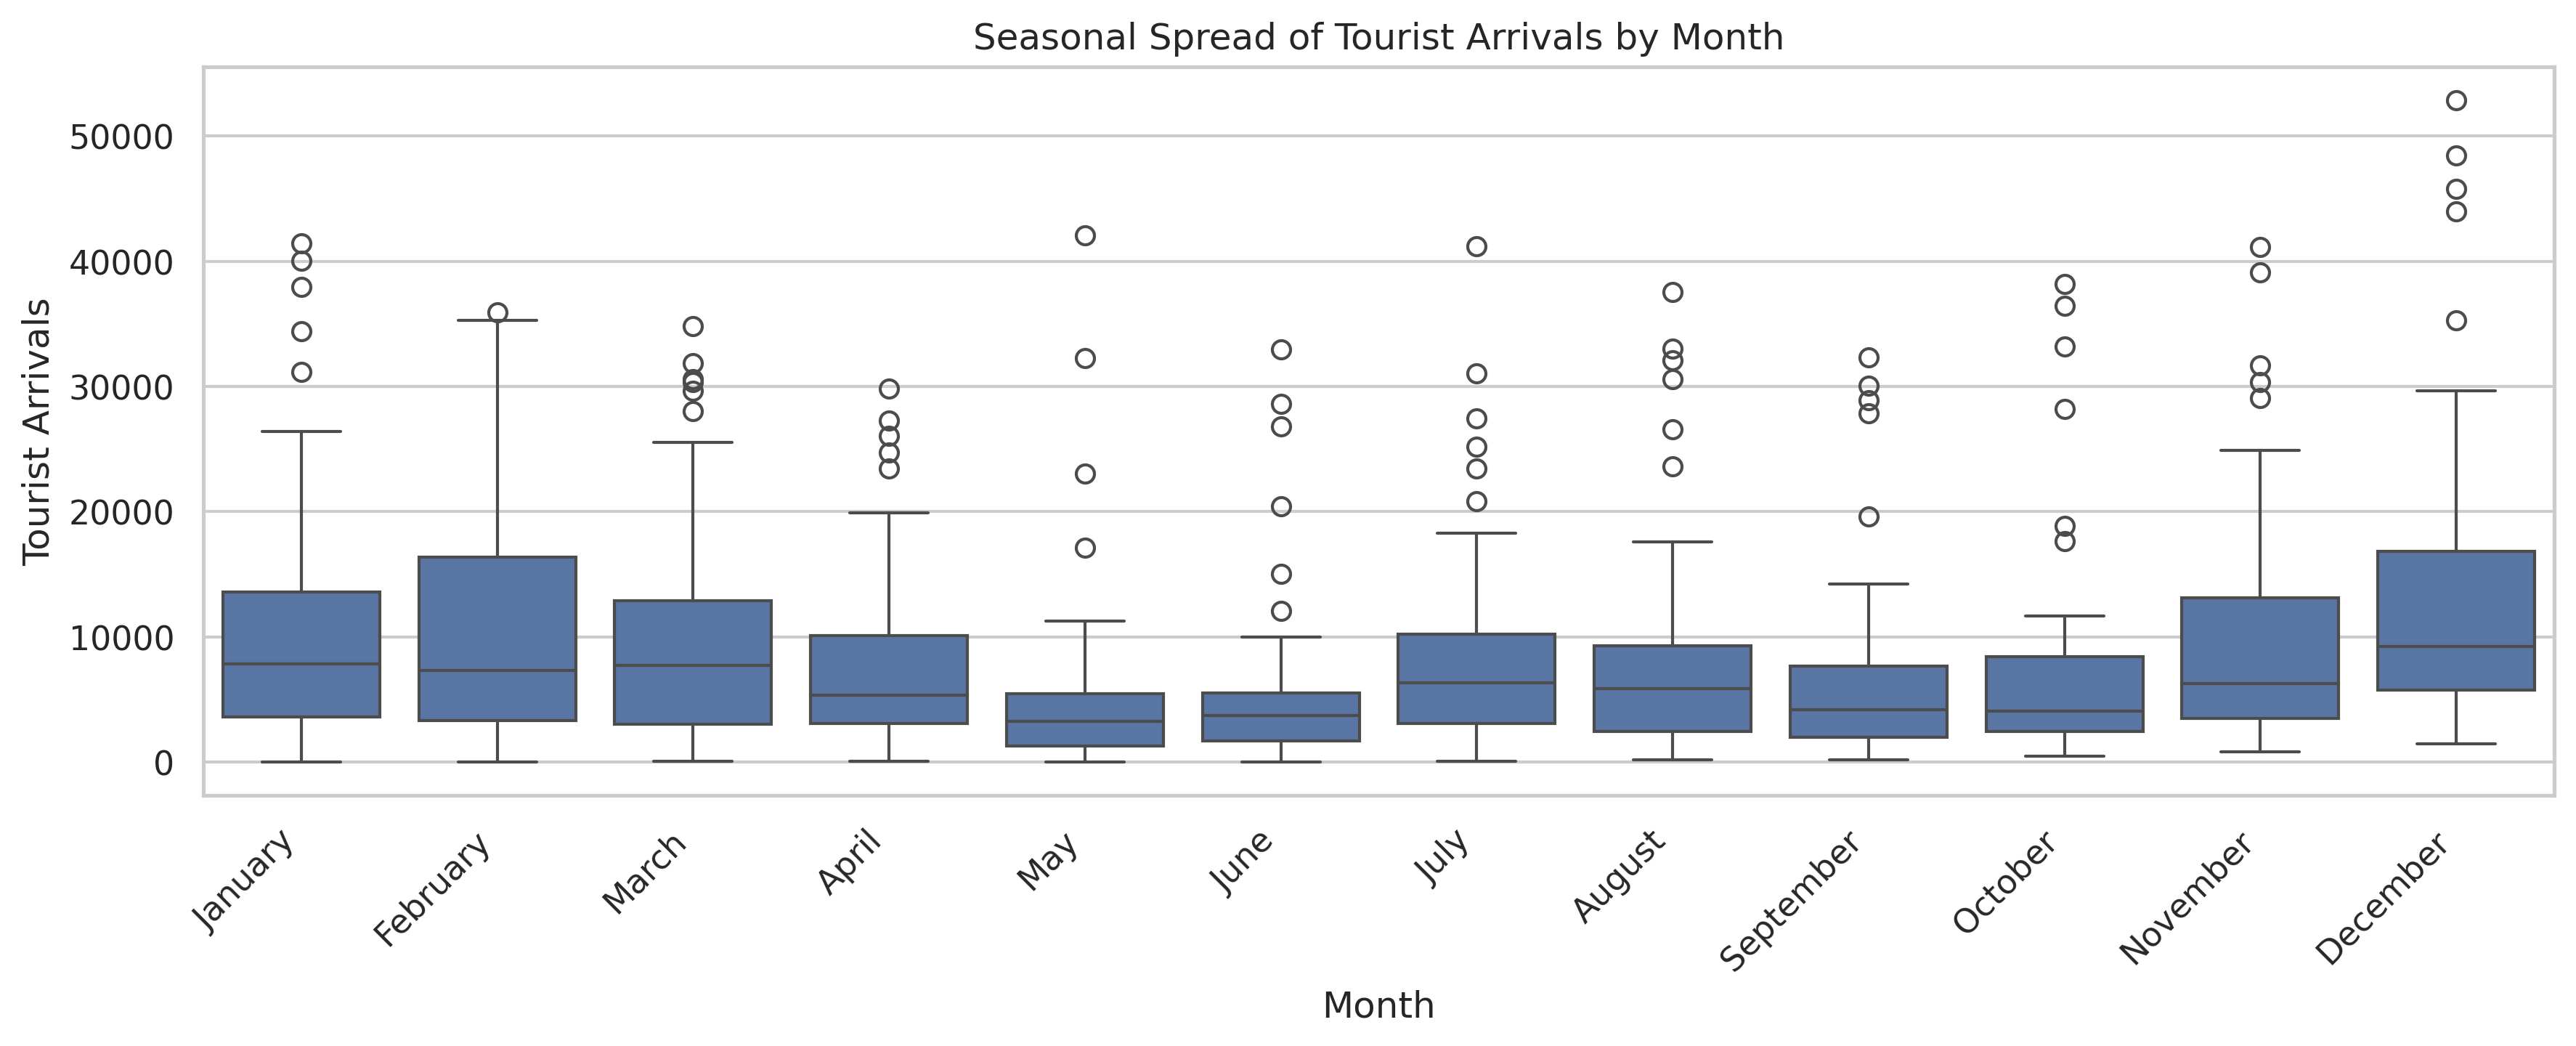
\includegraphics[width=\columnwidth]{figures/monthly_arrivals_boxplot.png}
\caption{Seasonal distribution of tourist arrivals across calendar months.}
\label{fig:seasonal-boxplot}
\end{figure}

\subsection{Data Preparation}
The original numerical \texttt{year} feature was retained as a model input. A separate calendar-date column was derived from year and month only for chronological splitting and visualization, and only this derived date column was excluded from modeling. Therefore, the full model retained all 12 original predictors: 10 numerical features and two categorical features. Month names were converted to their calendar positions. Numerical predictors were standardized, while month and origin country were one-hot encoded; unknown categories were ignored so that the pipeline could process future data. In the chronological training set, one-hot encoding expanded the 12 raw inputs to 49 transformed features for Linear Regression and SVR. Polynomial Regression produced 39 transformed features because month was represented by two scaled polynomial terms rather than 12 one-hot month indicators. These transformations were fitted using only the training subset through a scikit-learn pipeline \cite{pedregosa2011sklearn}, reducing the risk of data leakage.

The primary chronological split used 2018--2022 for training, 2023 for validation, and 2024 for testing (Table~\ref{tab:dataset-split}). A random 70/15/15 split measured interpolation but was considered optimistic for future forecasting. A reduced Linear Regression experiment retained month, country, and six numerical predictors with absolute target correlation of at least 0.15, giving eight raw features.

The preprocessing pipeline was fitted independently within each training partition. Consequently, numerical scaling parameters and one-hot-encoding categories were learned without using the corresponding validation or test targets. The target distributions across the chronological partitions were also examined to assess temporal stability. The higher target level and changed spread in the validation and test periods provide further evidence of distribution shift during the later stages of tourism recovery.

\subsection{Regression Models}
Linear and polynomial regression provide standard supervised-learning baselines \cite{hastie2009elements}. For a feature vector $\mathbf{x}$, the linear prediction is
\begin{equation}
    \hat{y}=\beta_0+\sum_{j=1}^{p}\beta_j x_j,
\end{equation}
where $\beta_0$ is the intercept and $\beta_j$ denotes the coefficient associated with predictor $x_j$.

Polynomial Regression was used to examine whether a simple nonlinear seasonal relationship improved prediction. A second-degree polynomial expansion was applied only to the month variable, while the remaining numerical and categorical predictors were processed in the same manner as in the linear pipeline. Restricting the expansion to month avoided a large number of unstable interaction terms in this relatively small dataset. Both linear estimators used ordinary least squares with the default scikit-learn settings.

SVR with an RBF kernel was included as a more flexible nonlinear alternative \cite{smola2004svr}. SVR seeks a function whose deviations from the observed targets remain within an $\epsilon$-insensitive margin while penalizing deviations outside that margin. The experiment used $C=10$ and $\epsilon=0.1$. Because SVR is sensitive to scale, the input predictors were processed using the same standardization and encoding pipeline as Linear Regression, and the target variable was standardized during fitting through a transformed-target regressor. Predictions were then automatically returned on the original arrival-count scale. No hyperparameter search was performed, so the reported SVR results apply specifically to this configuration.

\subsection{Evaluation Metrics}
Performance was evaluated using MAE, MSE, RMSE, and $R^2$, as required for a regression problem. For $n$ observations with actual values $y_i$ and predictions $\hat{y}_i$, MAE and RMSE are defined as
\begin{align}
    \mathrm{MAE} &= \frac{1}{n}\sum_{i=1}^{n}|y_i-\hat{y}_i|,\\
    \mathrm{RMSE} &= \sqrt{\frac{1}{n}\sum_{i=1}^{n}(y_i-\hat{y}_i)^2}.
\end{align}
Lower MAE, MSE, and RMSE values indicate smaller prediction errors. The $R^2$ score measures the proportion of target variance explained relative to predicting the subset mean; values closer to one indicate a better fit.

\section{Results}

\subsection{Model Performance}
Table~\ref{tab:model-performance} summarizes chronological model performance. Linear Regression produced the lowest validation and test RMSE values and the highest $R^2$ scores. On the 2024 test subset, it explained approximately 54.6\% of the observed variance. Polynomial Regression achieved the lowest test MAE, but its higher RMSE indicates that some of its errors were larger. SVR was the weakest model on both chronological subsets: its negative $R^2$ values show that it performed worse than predicting the mean arrival count of each evaluation subset.

\begin{table*}[htbp]
\caption{Regression Model Performance on Chronological Split}
\label{tab:model-performance}
\centering
\begin{tabular}{llrrrr}
\toprule
\textbf{Model} & \textbf{Subset} & \textbf{MAE} & \textbf{MSE} & \textbf{RMSE} & \textbf{$R^2$} \\
\midrule
Linear Regression & Validation 2023 & 4,819.65 & $4.684\times10^7$ & 6,844.24 & 0.256 \\
Linear Regression & Test 2024 & 5,011.12 & $4.528\times10^7$ & 6,729.14 & 0.546 \\
Polynomial Regression & Validation 2023 & 5,998.05 & $6.243\times10^7$ & 7,901.21 & 0.008 \\
Polynomial Regression & Test 2024 & 4,786.24 & $5.196\times10^7$ & 7,208.48 & 0.479 \\
Support Vector Regression & Validation 2023 & 5,564.25 & $7.242\times10^7$ & 8,510.18 & $-0.151$ \\
Support Vector Regression & Test 2024 & 7,769.74 & $1.467\times10^8$ & 12,111.04 & $-0.470$ \\
\bottomrule
\end{tabular}
\end{table*}

Table~\ref{tab:random-performance} presents the secondary random-split experiment. All three models obtained higher $R^2$ scores than in chronological testing. The difference was greatest for SVR, whose test $R^2$ increased from $-0.470$ under chronological evaluation to 0.835 under random evaluation, while its RMSE decreased from 12,111.04 to 4,064.67. In the random experiment, SVR was the strongest model on both validation and test subsets. This reversal demonstrates that the estimated model quality depends strongly on whether the evaluation requires extrapolation to a future year or interpolation among randomly held-out historical observations.

\begin{table*}[htbp]
\caption{Model Performance with a Random 70/15/15 Split}
\label{tab:random-performance}
\centering
\begin{tabular}{llrrrr}
\toprule
\textbf{Model} & \textbf{Subset} & \textbf{MAE} & \textbf{MSE} & \textbf{RMSE} & \textbf{$R^2$} \\
\midrule
Linear Regression & Validation & 3,893.74 & $2.936\times10^7$ & 5,418.66 & 0.721 \\
Linear Regression & Test & 3,950.72 & $3.043\times10^7$ & 5,516.05 & 0.696 \\
Polynomial Regression & Validation & 4,128.26 & $3.167\times10^7$ & 5,628.00 & 0.699 \\
Polynomial Regression & Test & 4,272.56 & $3.468\times10^7$ & 5,889.12 & 0.653 \\
Support Vector Regression & Validation & 2,887.23 & $1.914\times10^7$ & 4,374.85 & 0.818 \\
Support Vector Regression & Test & 2,901.56 & $1.652\times10^7$ & 4,064.67 & 0.835 \\
\bottomrule
\end{tabular}
\end{table*}

The full Linear Regression model outperformed the reduced alternative: test RMSE rose from 6,729.14 to 11,944.06 and $R^2$ fell from 0.546 to $-0.430$, showing that weakly correlated variables can still provide useful joint information.
Fig.~\ref{fig:split-comparison} visualizes the effect of evaluation strategy. All models improve under random testing, but SVR exhibits the largest change. Its strong random performance and weak chronological performance indicate sensitivity to the difference between interpolation within familiar historical regimes and extrapolation to a later recovery regime.

\begin{figure*}[htbp]
\centering
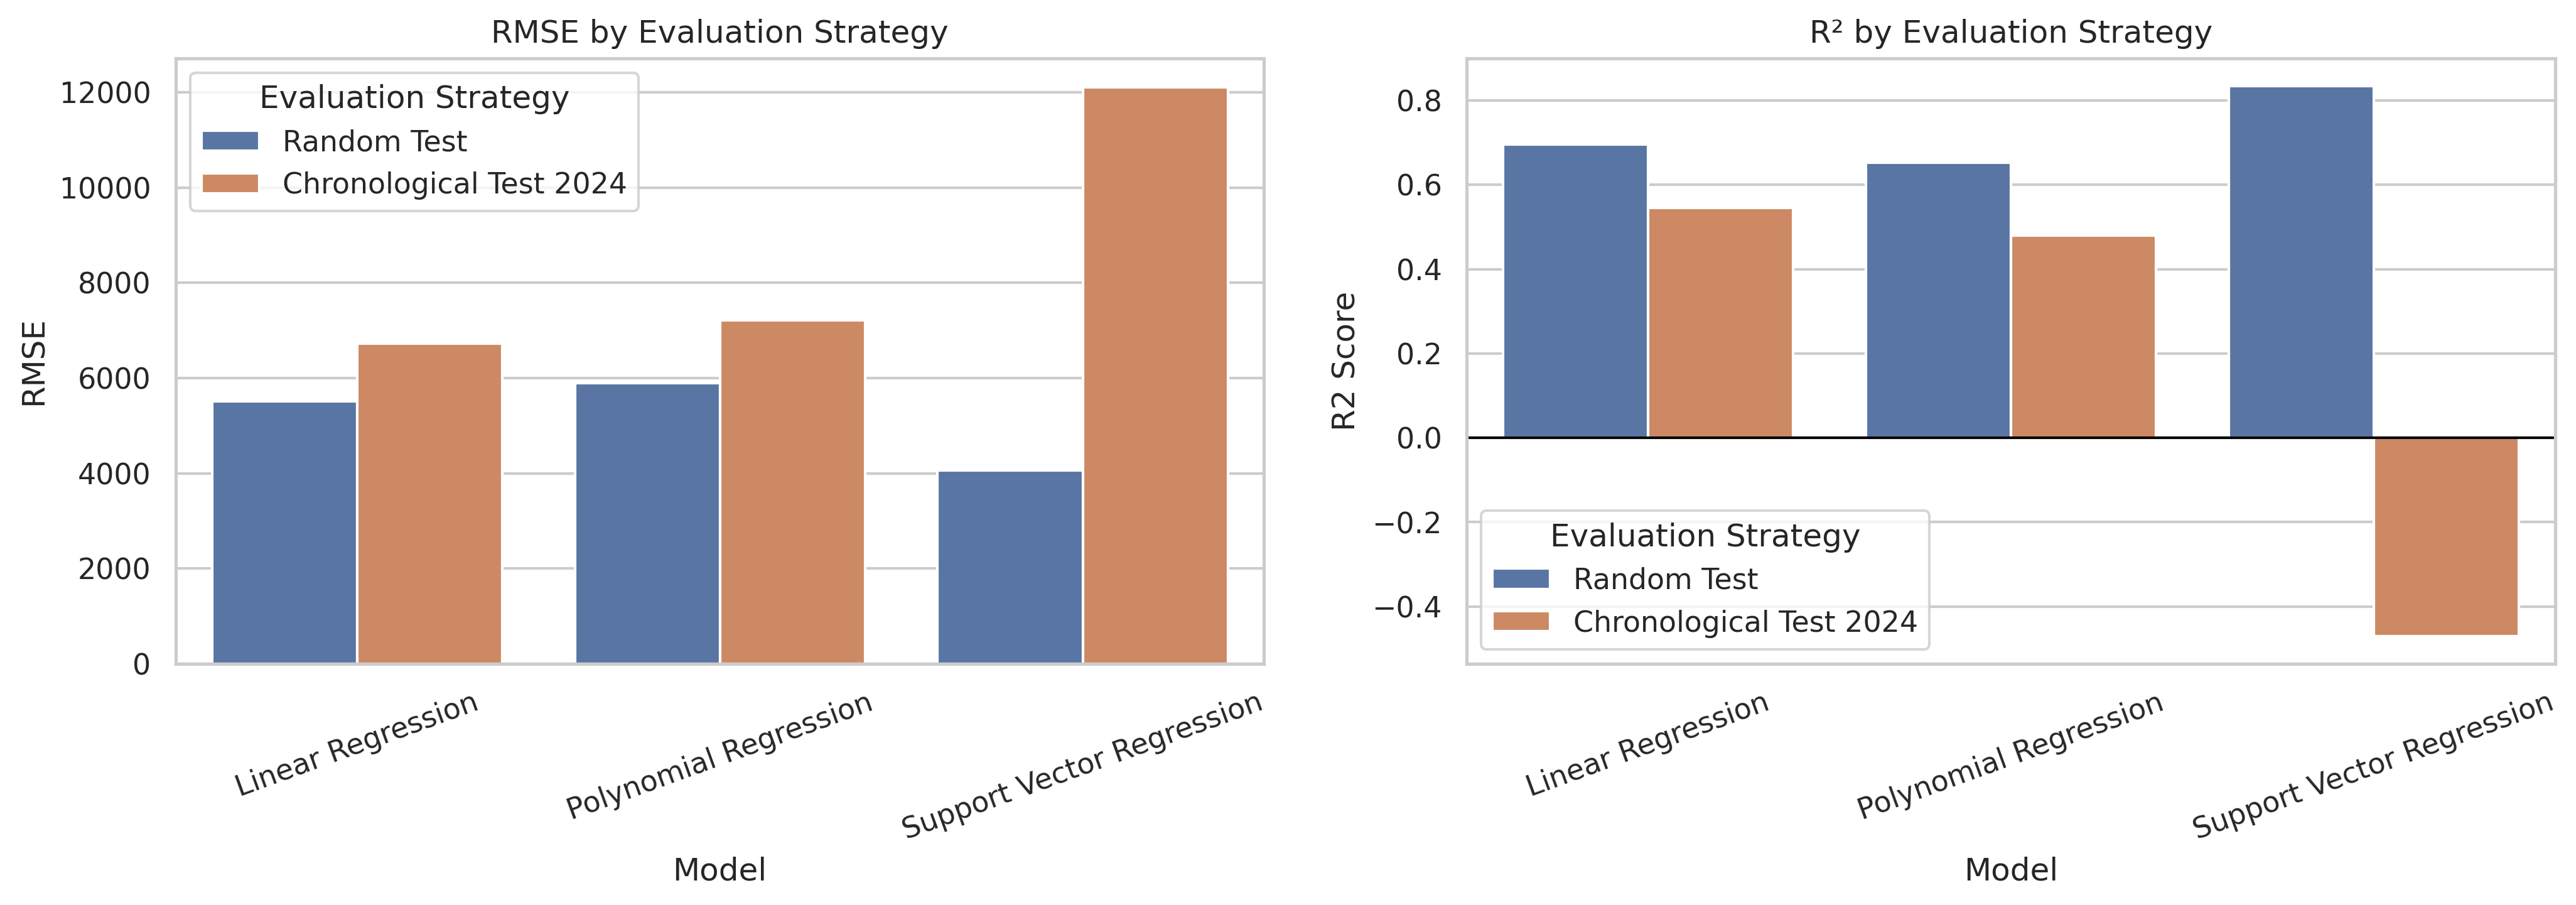
\includegraphics[width=0.9\textwidth]{figures/split_strategy_comparison.png}
\caption{RMSE and $R^2$ comparison for chronological and random test strategies.}
\label{fig:split-comparison}
\end{figure*}

\subsection{Interpretation of Results}
The more consistent forecasting across both chronological holdout years over the time period led to the selection of Linear Regression as the better forecasting model. This indicates a little useful explanatory power from the added quadratic month term in 2023 because the validation $R^2$ of the Polynomial Regression model is low at 0.008. Its lower test MAE but higher test RMSE further suggests uneven performance: it may improve typical predictions while producing several comparatively large errors. SVR deteriorated from a chronological validation RMSE of 8,510.18 to a test RMSE of 12,111.04. Its 2024 $R^2$ of $-0.470$ indicates poor generalization to the latest year under the selected RBF-kernel settings, despite its strong random-test performance. More specifically, since $1-R^2=1.470$, the SVR's sum of squared prediction errors was approximately 1.47 times that of the test-set mean baseline. Thus, the negative value does not indicate an invalid metric; it indicates that the configured SVR was less accurate than assigning every 2024 observation the same mean value.

The relatively poor chronological $R^2$ values are largely attributable to a temporal distribution shift caused by COVID-19. The 2018--2022 training set is not governed by one stable tourism pattern: it contains relatively high pre-pandemic arrivals, a sharp collapse during the pandemic, and only the beginning of recovery. The 2023 validation set and 2024 test set instead represent later stages of recovery, during which arrivals increased gradually but followed a pattern different from both the pre-pandemic and pandemic periods. Consequently, the relationships between the year, economic variables, seasonal conditions, and arrivals differ substantially among the training, validation, and test sets. The models must extrapolate from this mixed training history to a new recovery regime, which increases error and reduces $R^2$.

Random splitting obscures much of this difficulty because it distributes observations from the pre-pandemic, pandemic, and recovery periods across all three subsets. Training can therefore contain rows that are temporally close to, and share month-year predictors with, validation and test rows. This makes the distributions more similar and explains why random-split scores are substantially higher. These scores are useful for measuring interpolation, but they are optimistic estimates of the ability to forecast a completely unseen future year.

The remaining error is substantial in practical terms. For example, the linear model underestimated January 2024 arrivals from India and Russia by approximately 6,092 and 16,850 visitors, respectively. Such errors indicate that origin-specific recovery patterns and external shocks are not fully represented by the available predictors. Consequently, the model is more suitable as a baseline for comparative analysis than as a stand-alone operational forecasting system.

\section{Discussion}
The results show that additional model complexity does not necessarily improve future-year forecasting performance. A single quadratic representation of month cannot adequately describe structural changes across years or differences among origin countries. Similarly, an RBF kernel primarily interpolates among patterns represented in its training feature space and does not naturally extend a rising temporal trend beyond that space. It therefore did not extrapolate effectively from the mixed pre-pandemic, pandemic, and early-recovery training patterns to the later recovery years. The contrast between SVR's chronological test $R^2$ of $-0.470$ and random-test $R^2$ of 0.835 is particularly informative. It shows that SVR can fit nonlinear relationships when training and testing come from similar mixed-period distributions, but performs poorly when required to generalize to a temporally different regime. This limitation may be intensified by the relatively small sample, one-hot-encoded country feature space, absence of lagged arrival predictors, and use of fixed $C$, $\epsilon$, and kernel-width settings without time-aware hyperparameter tuning. The result should therefore not be interpreted as evidence that SVR is unsuitable for tourism prediction in general. Conversely, the full linear model benefits from using the complete collection of economic, weather, capacity, and categorical variables, even though the pairwise numerical correlations with the target are weak.

A strength of the study is its leakage-aware chronological evaluation together with an explicit random-split comparison. The comparison demonstrates why a favorable random score should not automatically be reported as forecasting performance. Comparable preprocessing pipelines are applied consistently, the SVR target is scaled using training data, and all four regression metrics required by the assignment are reported. Linear Regression also provides a transparent baseline that can be reproduced and interpreted readily.

The study has several limitations. First, 750 observations constitute a relatively small sample, particularly after reserving complete years for validation and testing. Second, the dataset includes the exceptional disruption and recovery associated with COVID-19, but the current features do not explicitly represent travel restrictions or crisis periods. Third, several predictors vary by month or year rather than by origin country, which limits their ability to explain country-level differences. Finally, the analysis establishes predictive association rather than causation.

Future work could add lagged arrival counts, public holidays, events, travel-restriction indicators, flight capacity, and origin-specific macroeconomic variables. If permitted by the course scope, SVR could also be tuned on the validation period by testing $C$, $\epsilon$, and kernel-width values without using the test set for model selection. Any additional algorithms should remain within those covered in the course and should be compared using the same chronological partitions.

\section{Conclusion}
This study established an initial machine-learning approach for predicting tourist arrivals to Sri Lanka using a combination of temporal, origin-country, economic, environmental, and tourism-capacity features. Linear Regression, second-degree Polynomial Regression, and RBF-kernel SVR were evaluated using both chronological and random data partitions. Under the primary chronological design, Linear Regression achieved the strongest overall generalization, with a 2024 test RMSE of 6,729.14 and an $R^2$ score of 0.546, while SVR produced an RMSE of 12,111.04 and an $R^2$ of $-0.470$. Under random testing, SVR achieved a substantially stronger RMSE of 4,064.67 and an $R^2$ of 0.835. This difference shows that random splitting creates a much easier interpolation task by mixing pre-pandemic, pandemic, and recovery observations across the subsets. Chronological evaluation, on the other hand, reveals the COVID-related structural break: the distribution of tourism collapsed and then slowly rebounded following a different pattern, thus resulting in significantly different distributions for the training, validation, and test sets. Thus, the chronological results give a more reliable prediction of the forecasting performance of the future years. While the linear model accounts for a significant fraction of the variation in arrivals, the level of error in the model, and the significant changes in the study period indicate a need for more detailed time-dependent, crisis-related, and country-specific predictors to ensure reliable operational forecasts.

\section*{Acknowledgment}
The author sincerely thanks Eng. S. U. Dampage, lecturer for the ET-3043 Machine Learning module, for his clear instruction, practical insights, and continued encouragement throughout this project. Appreciation is also extended to the author's batchmates for their collaboration, constructive discussions, and support in overcoming challenges during the learning process.

\bibliographystyle{IEEEtran}
\bibliography{references}

\end{document}
